\testCom
{%Номер задачи
	3.125
}
{%Условие
	условие
}
{%Дано
	дано
}
{%Найти
	найти
}
{%Решение
	%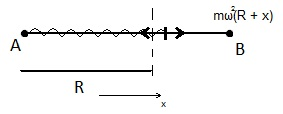
\includegraphics[height=30mm]{3_33.jpg}\\
	$U(t) = U e^{- \beta t} \cos \omega t$\\
	a) $\abs{\cos \omega t_A} = 2 \Rightarrow \omega t_A = \pi n \quad t_A = \frac{\pi n}{\omega}$\\
	б) $\der{U}{t}{} = - e^{- \beta t} (\omega \sin \omega t_0 + \beta \cos \omega t_0) = 0$\\
	$- e^{- \beta t} \cdot \frac{1}{\sqrt{\omega^2 + \beta^2}} \cos (\omega t_0 - \varphi) 0 = - e^{- \beta t} \sin (\omega t_0 + \varphi)$\\
	$\varphi = \arccos \frac{\omega}{\sqrt{\omega^2 + \beta^2}} = \arctg \frac{\beta}{\omega}$\\
	$\omega t_0 + \varphi = \pi n \quad t_0 = \frac{\pi n - \varphi}{\omega} = \frac{\pi n - \arctg \frac{\beta}{\omega}}{\omega}$\\
}

